\chapter{Meditation Requires Order}

Meditation is named at the beginning, but it is not treated as a technique. Krishnamurti asks what must be true of the mind for meditation to be real, and then he delays the answer. Freedom, violence, choice, psychological time, disorder, love, and death have to be examined first. The structure of the lecture is therefore not a list of topics. It is a sequence of obstructions being removed before meditation can be understood as something other than escape.

The notation in this chapter is only schematic. There is no blackboard mathematics in this lecture, and no validated visual frame carries an equation or diagram. The symbols and figures below are compact reconstructions of the spoken argument, meant to make the distinctions visible without replacing the inquiry itself.

\section{Meditation Begins With Freedom}

The first question is not, ``How do we meditate?'' It is more radical: what is necessary for a mind that is capable of true meditation? The first step, Krishnamurti says, is to understand freedom.

Freedom immediately divides into two different things. There is outward freedom: political freedom, freedom to express oneself, freedom to think what one likes, freedom to choose, freedom from a particular habit. And there is inward freedom: freedom from the mind's own projections, demands, desires, fulfilments, cravings, and appetites.

The first distinction can be written as
\begin{equation}
F_{\mathrm{out}} \not\Rightarrow F_{\mathrm{in}} .
\end{equation}
This is not a theorem from the lecture. It is a compact way to keep the first move clear: outward freedom is necessary in its own field, but it does not by itself make the mind inwardly free.

\begin{definition}
Let \(F_{\mathrm{out}}\) denote outward freedom: political, social, expressive, and choice-based freedom. Let \(F_{\mathrm{in}}\) denote inward freedom: freedom from projection, craving, appetite, violence, fear, dependence, authority, and conditioning.
\end{definition}

The lecture grants political freedom its place. One must have it. But then it asks why we do not ask with the same intensity whether inward freedom is possible. A mind may be allowed to choose outwardly while remaining a slave to its own movement.

This is why meditation cannot begin as a method. If the mind is not free, a method only gives the unfree mind another pattern to obey.

\section{Choice, Violence, And The Verb To Be}

The next step overturns a common assumption. We usually regard choice as a mark of freedom. Krishnamurti treats psychological choice as a sign that the mind does not see clearly. When there is clear seeing, there is no inner bargaining; there is only action.

The spoken movement can be summarized as
\begin{align}
\mathrm{Clarity}
&\Rightarrow \mathrm{No\ Choice}
\Rightarrow \mathrm{Action}, \\
\mathrm{Choice}
&\Rightarrow \mathrm{Confusion}
\Rightarrow \mathrm{Resistance/Conflict}.
\end{align}
The notation should remain subordinate to the statement. The point is not that all practical selection is confused. The point is that inward choice, as the lecture uses the word, belongs to a divided mind.

\subsection{Question \& Answer}

\paragraph{Question.}
If choice usually looks like freedom, why does Krishnamurti say that choice indicates a lack of freedom?

\paragraph{Answer.}
Because he is speaking about the mind that chooses from confusion. When the mind sees clearly, it does not set up alternatives and then select among them. The seeing itself acts. But when the mind is uncertain, divided, or unclear, it chooses, resists, compares, and enters conflict. In that sense, choice is not freedom; it is evidence that freedom is absent.

The lecture then widens the meaning of violence. Violence is not only war, aggression, or social revolt. It is also the inward structure of resistance and conflict. A society that concentrates on outward change without inward change carries violence in another form.

We may mark that enlarged field by
\begin{equation}
\mathrm{Violence} \supset
\{\mathrm{choice},\ \mathrm{conflict},\ \mathrm{outward\ change\ without\ inward\ change}\}.
\end{equation}
This is an editorial set relation, not a definition. It preserves the lecture's insistence that violence is woven into the ordinary movement of the mind.

Then the argument goes deeper. Our life, Krishnamurti says, is conditioned by the verb ``to be.'' The mind is organized by becoming:
\begin{equation}
\mathrm{To\ Be}:\qquad
\mathrm{has\ been} \longrightarrow
\mathrm{is} \longrightarrow
\mathrm{will\ be}.
\end{equation}
In that verb lie the ideas of arriving, succeeding, achieving, becoming, gradually attaining peace, and gradually getting rid of what hinders us. The moral structure of the mind is built in the same pattern: I will be good; I will gradually achieve a certain state.

That movement is the conditioning of the mind in time.

\section{Time As Becoming}

The critique of psychological time is the hinge of the lecture. It connects choice and violence with the false map of spiritual progress. If the mind says, ``I will gradually become peaceful,'' it has already accepted the structure of becoming. It has placed freedom, order, love, or enlightenment in the future.

The counterclaim can be written schematically:
\begin{equation}
\mathrm{Understanding} \neq
\lim_{t\to\infty}\mathrm{Gradual\ Improvement}(t).
\end{equation}
The equation is not meant as formal mathematics. It gives shape to the spoken point: understanding is not the limit of accumulated improvement. Enlightenment is not a matter of time. Either there is direct understanding, or there is not.

\subsection{Question \& Answer}

\paragraph{Question.}
Can understanding be gradual?

\paragraph{Answer.}
The lecture says no, if by gradual we mean psychological becoming through time. Gradual skill has its place in practical matters, but understanding in this inquiry is not a product of accumulation. The mind that says, ``I will understand later,'' is still moving within the verb ``to be.'' It has turned understanding into a future state.

This is why the word itself becomes dangerous. The word is not the thing; the description is not the described. Yet the mind is satisfied with descriptions, explanations, and promises of arrival.

At this point meditation returns, but only to be postponed again. Before one can understand meditation, one must understand living, love, and death. Without that foundation, meditation is merely escape or self-hypnosis.

\section{Living As Disorder}

The foundation is not an idea of order. The foundation is the observation of actual life. The lecture now turns from the abstract structure of becoming to the ordinary life we live every day.

That life is described as disorder: conflict, driving ambition, battle within oneself, opposing desires and wills, frustration, comparison, escape, loneliness, routine, division, and self-centred activity. The centre that wants fulfilment is itself questioned. Is not that centre the cause of disorder?

A central opposition appears:
\begin{equation}
\mathrm{What\ Is} \neq \mathrm{What\ Should\ Be}.
\end{equation}
When the mind lives between these two poles, it generates conflict:
\begin{equation}
\mathrm{Conflict}(\mathrm{What\ Is},\mathrm{What\ Should\ Be})
\Rightarrow
\mathrm{Disorder}.
\end{equation}

This gives us the first worked example in the chapter.

\begin{proof}
Suppose the mind observes its actual state: ambition, fear, envy, loneliness, frustration, or dependence. If it immediately compares that fact with an ideal state, what should be, it has introduced an opposing image. The actual fact and the projected image now stand against one another. That opposition is conflict. Since this conflict is the ordinary movement of daily life, the life itself is disorder.
\end{proof}

Krishnamurti uses the phrase ``complete mathematical order,'' but it should not be turned into technical mathematics. The word ``mathematical'' here points to completeness and precision: order is not partial, decorative, imposed, or merely outward. Without order in the actual life one lives, meditation has no foundation.

The long inventory of disorder prepares the next question.

\subsection{Question \& Answer}

\paragraph{Question.}
How can such a life be changed?

\paragraph{Answer.}
Not gradually. If change is postponed into gradual becoming, the same structure of time and violence continues. Change begins with seeing the fact non-verbally, not as an explanation or an idea, but as directly as one feels hunger. One must be intimately related to what is, without escape and without distortion.

\section{Observation, Discipline, And Order}

The central relation is now visible. Order is not imposed on disorder. Order arises from observing disorder without choice and without distortion.

The movement is
\begin{align}
\mathrm{Observation}_{\mathrm{no\ choice,\ no\ distortion}}(\mathrm{Disorder})
&\Rightarrow \mathrm{Learning}, \\
\mathrm{Learning}
&\Rightarrow \mathrm{Discipline}, \\
\mathrm{Discipline}
&\Rightarrow \mathrm{Order}.
\end{align}

The word discipline has to be rescued from its ordinary associations. It does not mean conformity, imitation, suppression, or obedience to an imposed pattern. It means learning. In the very act of observing, the mind learns, and that learning has its own discipline.

\begin{figure}
\centering
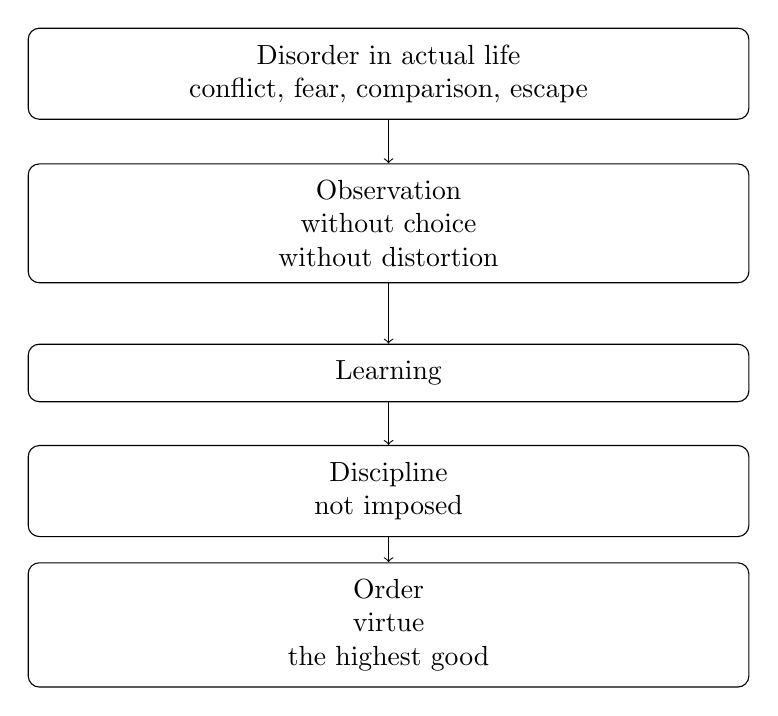
\begin{tikzpicture}[
  box/.style={draw, rounded corners, align=center, text width=0.72\linewidth, inner sep=6pt}
]
\node[box] (d) at (0,0) {Disorder in actual life\\conflict, fear, comparison, escape};
\node[box] (o) at (0,-1.9) {Observation\\without choice\\without distortion};
\node[box] (l) at (0,-3.8) {Learning};
\node[box] (disc) at (0,-5.3) {Discipline\\not imposed};
\node[box] (ord) at (0,-7.0) {Order\\virtue\\the highest good};
\draw[->] (d) -- (o);
\draw[->] (o) -- (l);
\draw[->] (l) -- (disc);
\draw[->] (disc) -- (ord);
\end{tikzpicture}
\caption{A transcript-backed reconstruction of the lecture's movement from observed disorder to order.}
\end{figure}

The decisive point is subtle. If we try to bring order out of disorder by imposing what we think order should be, we create another conflict between what is and what should be. That is still disorder. The observation has to be choiceless; otherwise the observer is already selecting, resisting, and distorting.

The lecture then turns outward for contrast. Revolutions try to establish outward order first. They change one system for another, or insist on state order, while neglecting inward order. Krishnamurti says this has never solved the problem.

We can express the asymmetry as
\begin{equation}
\mathrm{Inward\ Order} \Rightarrow \mathrm{Outward\ Order},
\qquad
\mathrm{Outward\ Order} \not\Rightarrow \mathrm{Inward\ Order}.
\end{equation}
The order required for meditation is therefore not state order, social discipline, or imposed morality. It is the order that comes when disorder is seen without distortion.

\section{Love Through Negation}

From order the lecture moves to love. This is not a soft transition. If order is the ending of inward conflict, and if conflict is bound up with comparison, fear, and self-centred activity, then love cannot be understood apart from order.

Krishnamurti asks, ``What is love?'' and immediately refuses to define it positively. The way is through negation: find out what it is not.

\begin{equation}
\mathrm{Love} \notin
\{\mathrm{jealousy},\mathrm{envy},\mathrm{comparison},\mathrm{pleasure},
\mathrm{dependence},\mathrm{fear},\mathrm{authority},\mathrm{conditioning}\}.
\end{equation}
This is not a complete definition of love. It is a compact record of the exclusions by which the lecture proceeds.

\subsection{Question \& Answer}

\paragraph{Question.}
Can love be cultivated?

\paragraph{Answer.}
No. Cultivation belongs to thought and becoming. A proud mind that cultivates humility remains proud in the very act of cultivation. In the same way, a mind that sets out to cultivate love is still operating through projection, time, and the desire to become. The lecture therefore asks us to see what love is not, and to let the false disappear in the seeing.

The first negations are jealousy and envy. Love hedged about by jealousy is not love. Envy comes with comparison, and the lecture asks whether love can be comparison. If comparison is seen and ends, envy loses its ground.

The harder negation is pleasure. Pleasure is sustained by thought. A remembered experience is carried over; thought builds image upon image; the image stimulates; and that stimulation is called pleasure. The process may be shown as
\begin{equation}
\mathrm{Remembered\ Experience}
\xrightarrow{\ \mathrm{thought}\ }
\mathrm{Image\ upon\ image}
\xrightarrow{\ \mathrm{stimulation}\ }
\mathrm{Pleasure}.
\end{equation}

The lecture does not deny enjoyment. It questions the psychological machinery that turns memory, image, dependence, and fear into what we call love. In pleasure there is frustration, pain, agony, and dependence. In dependence there is fear.

A short derivation keeps the sequence clear:
\begin{align}
\mathrm{Pleasure\ as\ image}
&\Rightarrow \mathrm{Dependence}, \\
\mathrm{Dependence}
&\Rightarrow \mathrm{Fear}, \\
\mathrm{Pleasure\ as\ image}
&\Rightarrow \mathrm{Fear}.
\end{align}
This is a worked logical chain, not a psychological theory added from outside. It follows the lecture's order: thought sustains pleasure, pleasure carries dependence, dependence contains fear, and what contains fear cannot be love.

The inquiry then widens again. We are conditioned by society, propaganda, education, books, authority, and memory. Experience itself is old if it is recognized, because recognition is the response of memory. Thought is old for the same reason. Thus the human being becomes second-hand: intellectually, emotionally, morally.

Love cannot be second-hand. It cannot come through authority, training, repetition, or the memory of what others have said.

\section{Death And The Ending Of The Known}

To understand love, the lecture says, one must also understand death. This is not a new subject placed beside the others. Living, love, and death are to be seen as one movement, not as three compartments.

The point may be written negatively:
\begin{equation}
\mathrm{Life} \neq
\{\mathrm{Living}\}\cup\{\mathrm{Love}\}\cup\{\mathrm{Death}\}
\quad \hbox{as separate compartments.}
\end{equation}
A better prose version is: life includes living, love, and death as a total movement.

Krishnamurti first acknowledges biological death. The organism comes to an end through age, disease, usage, accident, and the wear of conflict. But he does not stay with biological ending. He asks about the ending of the ``me,'' the centre that divides itself into us and they, we and you, and therefore becomes the centre of conflict.

\subsection{Question \& Answer}

\paragraph{Question.}
Can the ``me'' die, not eventually, but every day?

\paragraph{Answer.}
That is the lecture's practical question about death. To die every day is to end one's psychological accumulation: pleasure, knowledge, memory, and the furniture of the mind. It is not an idea about afterlife. It is the ending of the known in the present.

The distinction is
\begin{align}
\mathrm{Death}_{\mathrm{bio}}
&= \mathrm{Ending\ of\ the\ organism}, \\
\mathrm{Death}_{\mathrm{psych}}
&= \mathrm{Ending}(\mathrm{me},\mathrm{known},\mathrm{pleasure},\mathrm{accumulation}).
\end{align}

The discussion of reincarnation has one function here: it redirects attention to how one lives now. Belief in afterlife does not answer the question. Even if one believes in reincarnation, what matters is the present movement of thought, action, morality, fear, and attachment.

The final relation is
\begin{equation}
\mathrm{Ending\ the\ Known} \Rightarrow \mathrm{Innocence\ of\ Mind}.
\end{equation}
Only such a mind, emptied of the known, can come upon what Krishnamurti calls enlightenment. The phrase ``can come upon'' is important. Enlightenment is not presented as a result achieved by time, method, repetition, or effort.

\section{Summary}

The lecture begins with meditation and then refuses every shortcut to meditation. First comes freedom, but freedom is not choice. Choice belongs to confusion; clarity acts. Violence is not merely outward aggression but the inward movement of conflict, resistance, and outward change without inward transformation.

The deeper structure is the verb ``to be,'' the mind's movement through psychological time: has been, is, will be. As long as the mind is organized by becoming, it turns even goodness, order, love, and enlightenment into future achievements.

The foundation for meditation is therefore the understanding of actual living. Actual living is disorder when it is governed by conflict, comparison, escape, ambition, fear, and the division between what is and what should be. Such a life does not change gradually. It changes through observation without choice and without distortion. That observation is learning; learning is discipline; discipline is order.

Order then opens into love, and love is approached through negation. It is not jealousy, envy, comparison, pleasure, dependence, fear, authority, or second-hand conditioning. Finally, love cannot be separated from death. Death is not only the ending of the organism but the daily ending of the ``me,'' the known, pleasure, and accumulation. In that ending the mind becomes innocent, and only such a mind is capable of true meditation.